% Use only LaTeX2e, calling the article.cls class and 12-point type.

\documentclass[12pt]{article}

\usepackage[round,semicolon]{natbib}
\usepackage{etoolbox}
\AtBeginEnvironment{quote}{\singlespacing\tiny}
% Use times if you have the font installed; otherwise, comment out the
% following line.

% added by SKH
\usepackage{lineno}
%\linenumbers

\usepackage{times}
\usepackage{amssymb}
\usepackage{amsmath}

\usepackage[export]{adjustbox}

\usepackage{graphicx}
\graphicspath{ {images/} }

% for adjustwidth
\usepackage{changepage}

% The following parameters seem to provide a reasonable page setup.

\topmargin 0.0cm
\oddsidemargin 1cm
\textwidth 15cm 
\textheight 21cm
\footskip 1.0cm

\usepackage{newfloat}
\usepackage{amsmath}
\usepackage[labelfont=bf]{caption}
\usepackage{nameref}
\usepackage{rotating}
\usepackage{color}
\usepackage{float}

% allow bigger floats per here: https://tex.stackexchange.com/a/11382
\renewcommand{\topfraction}{.95}
\renewcommand{\bottomfraction}{.95}
\renewcommand{\textfraction}{.05}
\renewcommand{\floatpagefraction}{.95}
\renewcommand{\dbltopfraction}{.66}
\renewcommand{\dblfloatpagefraction}{.66}
\setcounter{topnumber}{9}
\setcounter{bottomnumber}{9}
\setcounter{totalnumber}{20}
\setcounter{dbltopnumber}{9}

\renewcommand{\figurename}{{}}
\renewcommand{\thefigure}{{Figure~\arabic{figure}}}

\renewcommand{\tablename}{{}}
\renewcommand{\thetable}{{Table~\arabic{table}}}

\newfloat{suppfile}{thp}{losuppfile}
\renewcommand{\thesuppfile}{Supplementary~file~\arabic{suppfile}}
\floatname{suppfile}{}

\newfloat{suppfig}{thp}{losuppfig}
\renewcommand{\thesuppfig}{Supplementary~figure~\arabic{suppfig}}
\floatname{suppfig}{}

%
\newfloat{supptable}{thp}{losupptable}
\renewcommand{\thesupptable}{Supplementary~table~\arabic{supptable}}
\floatname{supptable}{}
%

\renewcommand{\theequation}{Equation~\arabic{equation}}

\newcommand\skhcomment[1]{{\color{cyan}[#1]}}
\newcommand\jdbcomment[1]{{\color{red}[#1]}}


\usepackage{hyperref}
\hypersetup{colorlinks,citecolor=blue,linkcolor=blue,urlcolor=blue}
\hypersetup{colorlinks,citecolor=blue,linkcolor=blue,urlcolor=blue}

\usepackage{seqsplit}

\usepackage{array}
\newcolumntype{P}[1]{>{\raggedright\arraybackslash}p{#1}}

\newlength\Colsep
\setlength\Colsep{10pt}
\usepackage{multicol,caption}

\usepackage{lipsum}
\newenvironment{Figure}
  {\par\medskip\noindent\minipage{\linewidth}}
  {\endminipage\par\medskip}

\title{A Discrete-time Markov Process for Predicting Influenza Evolution.}
\author{Emily Brunelli$^*$, Gunnar Johnson$^*$, Jonathan Mah$^*$}
\date{Math 381, Summer 2018}

\begin{document}
\maketitle
\footnotesize{$^*$Denotes equal contribution to work}\\

\section{Abstract}
Several infectious and chronic diseases are caused by viruses known to escape the human immune response \citep{russell2014science}. A current problem in public health is our inability to reliably forecast the evolutionary behavior of these viruses, which leads to challenges in vaccine design and disease surveillance. Current predictive models for viral evolution employ a wide range of mathematical techniques to address this problem, ranging from maximum likelihood and statistical inference to combinatorial and random-walk approaches \citep{kosakovsky2005not}. Here, we investigate the use of a discrete-time Markov process to predict the evolutionary behavior of the H1 strain of Hemagglutinin based on changes in DNA over time. Additionally, we evaluate the ``evolutionary variability" of each site along the protein, and compare our results to past works from literature.

\clearpage

\begin{multicols}{2}


\section{Introduction}
Hemagglutinin is one of the two major proteins of the Influenza virus, and is mechanistically responsible for infecting the host cell \citep{wiley1987structure}. It is also a major target of the immune system and is known for having an abnormally high rate of evolution among viral proteins \citep{petrova2018evolution}. Many diseases such as polio and smallpox have been nearly eradicated due to successful attempts at vaccination, however, some viruses like Influenza continue to be able to escape long-term vaccination, most likely due to the extreme rate and diversity of its viral evolution. Due to both its medical and biological significance, influenza evolution is a common target for modern predictive algorithms \citep{morris2017predictive}. 

Recent advancements in computer science and discrete mathematics have revolutionized the study of molecular evolution, and as such, the application of predictive algorithms to evolution is relatively new. Contemporary efforts to predict influenza evolution often approach the problem through the lens of statistical phylogenetics. One such model, ``DEPS\footnote{Directional Evolution of Protein Sequences}" attempts to predict the directional evolution of each site in Hemagglutinin, that is, the rate of evolution as Hemagglutinin evolves towards a specific state \citep{kosakovsky2008maximum}. Other models such as the ``ExpCM\footnote{Experimentally Informed Codon Model}" incorporate a combination of experimental and computational approaches to measure the site-by-site variation of Hemagglutinin \citep{bloom2017identification}. These models provide a great deal of insight towards the evolutionary and immunological behavior of Influenza, however, the outright prediction of viral evolution is still a largely unsolved problem.

DNA nucleotides are chemical compounds which are analogous to machine code for biology \citep{hood2003digital}. DNA is first transcribed into an intermediate molecule known as RNA, which is then further translated into ``amino-acids" -- these ``amino-acids" form the individual components of proteins. The process by which DNA is transcribed into RNA and then translated into proteins is well studied, and as such we can directly map from length-3 sequences of DNA to the individual amino-acids of proteins \citep{searls1995string}. DNA possesses an inherently sequential structure, and as a result, by taking advantage of the linguistic characteristics of DNA, we can index specific sites along a protein relative to its overall structure \citep{brendel1986linguistics}. These observations form the current basis of the study of molecular evolution: changes in DNA result in changes in protein structure.

When indexed by site, we can detect the changes in the amino-acids of a protein \citep{kosakovsky2005not}. Changes between different amino-acids at a specific site along the protein are known as ``amino-acid substitutions". There are 20 unique amino-acids that each site can take on, which allows us to approximate each site as a independent system that can only take on one of twenty different states. By analyzing several years' worth of sequenced DNA, we are able to approximate the annual probability of amino-acid substitution for each site in a protein. Our goal is to investigate the use of these probabilities to construct a Markov Chain in order to model the behaviour of amino-acid substitution in Hemagglutinin -- which in effect will be an approximation for the behavior of influenza evolution. This model should provide insight into the evolutionary behavior of Hemagglutinin, and by extension, may also provide insight towards possible targets for vaccine design.

In \textit{Assumptions}, we detail the various assumptions and simplifications we made in designing the model. In \textit{Mathematical Model} we detail the methodology and design of our bioinformatics pipeline\footnote{The general methodology of bioinformatics is to develop a ``pipeline", which is a series of connected scripts that sequentially manipulate and analyze a given set of input data.}, as well as the format of the input, intermediate, and output data. In \textit{Solution of the Mathematical Problem} we discuss our application of a Markov Chain towards predicting future states of the model. In \textit{Testing} we discuss the accuracy of our model as compared to real data, as well as discuss various changes we made during the development process. In \textit{Results} we present our findings and compare them to past works from literature. In \textit{Improvements} we address the effect of the assumptions that we made as well as discuss potential improvements for future works. In \textit{Conclusion} we discuss the implications of our work as well as possible future directions for other similar projects.

\section{Assumptions}

\subsection{Site Independence}
In order for a Markov process to be used in our model, we treated each site as an independent system. In reality, it is very unlikely that the mutation of an individual site could be viewed as a completely independent event from the mutation of its neighbors \citep{fowler2014deep}. It is the combination of amino-acids in a protein that determines fitness, rather than the individual fitness of each site. By viewing each amino-acid site as independent, we lose the ability to detect the interference and interaction between sites\footnote{Amino-acids are chemicals, and as such are capable of reacting and interacting with other nearby amino-acids.}. Similarly, we also did not take into consideration epigenetic interactions\footnote{Not all of DNA is always ``used" in protein expression, and the control over whether certain regions of DNA are turned ``on" or ``off" is due to ``epigenetic interactions" \citep{liu2008gene}.}. For the purposes of simplifying the problem, we felt these were reasonable assumptions to make given our lack of computing resources and time. Additionally, the current state of DNA sequencing focuses on a technique known as ``deep mutational scanning", which analyzes the effect of every possible mutation at every site in a protein. However, this analysis is currently limited to only evaluating single sites at a time \citep{fowler2014deep}. Unpublished work in the Bloom Lab has found that analyzing multiple sites at the same time significantly increases run-time to the extent that this type of analysis is not currently computationally feasible.

\subsection{Dashes in FASTA format}
We made another major assumption when parsing our data. DNA sequencing is still a relatively new and imperfect process, and as a result, dashes (-) in a FASTA sequence are used to indicate that at least one error has occurred during sequencing \citep{harris2008single}. For example, dashes can represent gaps of indeterminate length. In other cases, for some extremely diverse viruses, like HIV, dashes can represent sites which have exhibited several different amino-acids and thus cannot be interpreted as possessing a single state. When there were dashes (-) in the FASTA files, we ignored that site in the sequence for that year. For example, if a sites history of amino-acids was $A \rightarrow - \rightarrow F \rightarrow K \rightarrow L \rightarrow - \rightarrow A$, then we treated it as $A \rightarrow F \rightarrow K \rightarrow L \rightarrow A$. This assumption was necessary, as we could not determine that actual amino acid represented by the dashes.

\subsection{Genetic Continuity}
Another assumption we made was the genetic continuity of our input data. Traditionally, the genetic history of an organism, known as its ``phylogeny" can be thought of as a binary tree, wherein the inner nodes represent the separation of two lineages. In Figure 1, we have shown an example phylogenetic tree of Influenza, as generated from the ``RAxML" software package \citep{stamatakis2006raxml}. In Figure 2, we've shown a close-up of the same phylogenetic tree.

\begin{Figure}
 \centering
 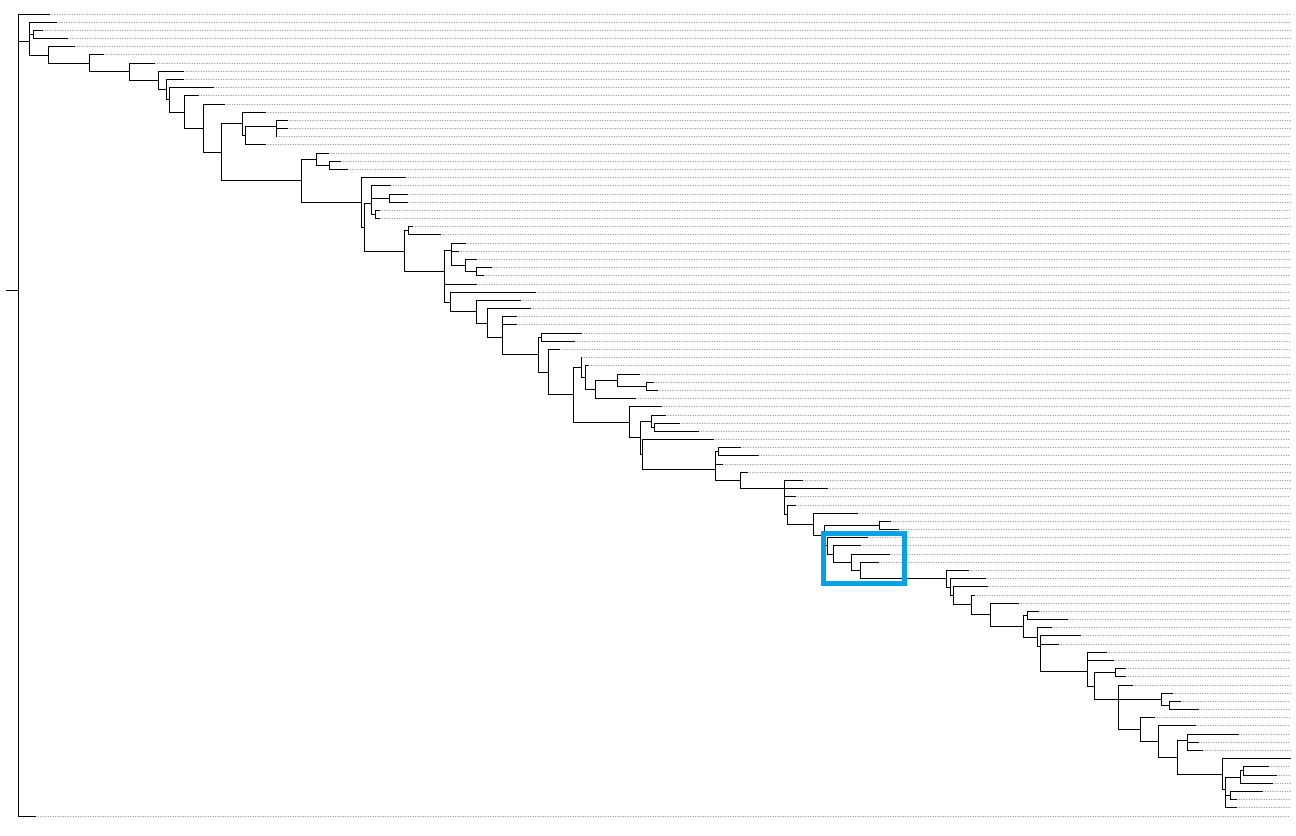
\includegraphics[width=\linewidth]{H1_Human_Subsample_0.png}
 \captionof{figure}{Example of Influenza Phylogeny}
\end{Figure}

\begin{Figure}
 \centering
 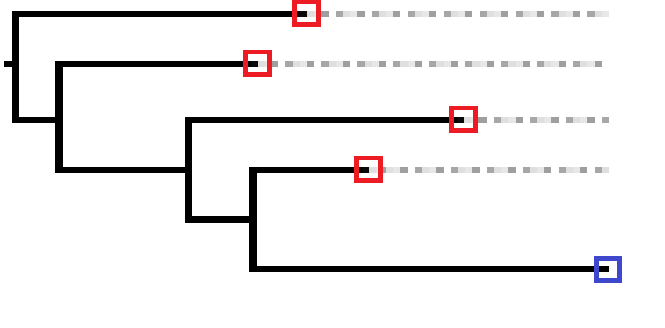
\includegraphics[width=\linewidth]{H1_Human_Subsample_0_closeUp.png}
 \captionof{figure}{Close-up of Influenza Phylogeny}
\end{Figure}

Influenza phylogenetic trees are known for resembling ``degenerate" binary trees, meaning that for every parent node, typically only one child node continues as a parent node \citep{taubenberger1997initial}. However, whenever we isolate and sequence a specific strain of DNA, we effectively end that lineage. This means that the sequences of Influenza that we analyzed are only ever the ending child nodes, which we've highlighted with red squares in Figure 2. Our model treats genetic history as linear in time, meaning that we assumed changes between red highlighted nodes would give insight towards the blue highlighted node. Additionally, our model is only capable of detecting the order of years sequenced -- the model is blind to the actual length of time between sequences, although most sequences are a year apart. As an analogy for human family trees, this would be similar to sequencing the DNA of aunts and uncles to try and predict the DNA of a niece. The impact of this assumption is somewhat diminished by taking smaller ``steps" in evolutionary history, as then our discrete process beings to resemble a continuous process. While unsuitable for humans, this assumption is generally considered acceptable for viruses, due to the relatively low genetic complexity of viruses, as well as the current limits of DNA sequencing. 

\subsection{Insertions and Deletions}
It is possible for mutations to occur in which the length of a DNA sequence increases or decreases by one nucleotide \citep{brendel1986linguistics}. The location of these aptly-named ``insertions" and ``deletions" can completely change how DNA is parsed and translated into amino-acids. If we allowed the length of input data to vary, we would not be able use a Markov chain, since the number of amino-acids would change and we would not longer by able to compare sites of corresponding index. To avoid this, we only used data with a length of 565 amino-acids.

\section{Mathematical Model}
Note that all data and scripts used in this analysis can be found on our team's GitHub\footnote{https://github.com/jon-mah/influenzaMarkov}. All input data was downloaded from the NCBI \citep{bao2008influenza}. We performed this analysis separately on five different input data sets.

\subsection{Markov Chain}

This application of Markov chains differs from the traditional approach in that we did not know the transition probabilities \textit{a priori} and as such had to construct the transition matrix from real data.

As input data, we used FASTA sequences, which take the following form:

\begin{Figure}
 \centering
 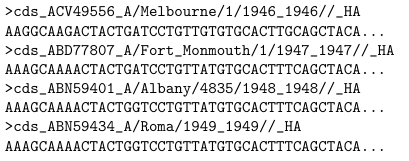
\includegraphics[width=\linewidth]{exampleInput.PNG}
 \captionof{figure}{Example input data}
\end{Figure}

In FASTA format, lines that begin with a ``$>$" contain information about the sequence that was isolated, (e.g., location, year, etc.). Using this information, we first sequentially ordered the data by the year that the strain was isolated. All other lines contain genetic information, usually shown as DNA nucleotides, which take the form of either ``A", ``C", ``G" or ``T".

We then converted the input data to FASTA sequences comprised of amino-acids. If DNA can be thought of as similar to machine code, then amino-acids can be thought of as compiled code. We decided to convert our sequences from DNA to amino-acids because amino-acids are more representative of protein function, and would likely give more insight towards the structure of H1 Hemagglutinin. This translation was performed according to the known mapping from nucleotides to amino-acids \citep{brendel1986linguistics}. This translation consists of mapping from length-3 sequences of DNA to site-indexed amino-acids:

\begin{Figure}
 \centering
 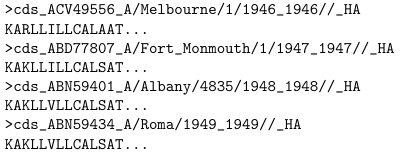
\includegraphics[width=\linewidth]{exampleIntermediate.PNG}
 \captionof{figure}{Example intermediate data}
\end{Figure}

This allows us to compare amino-acid sites of corresponding index between different sequences. For example, in Figure 4 , between the years of 1947 and 1948, the sixth amino-acid site mutated from ``I" to ``V". Using Python, we took a count of each mutation that occurred at every site, and found the sample probability of each transition, with the assumption that only the immediately preceding state could determine the next state.

From this, we generated a $20 \times 20$ Markov chain for the transition probabilities of each amino-acid site coded for by the Hemagglutinin gene. Hemagglutinin is a protein comprised of 565 amino-acids, so in effect, we constructed five hundred sixty-five $20 \times 20$ Markov chains.

The resulting probability matrices can be interpreted according to the following definitions: \\
\textbullet{} Each transition matrix represents the Markov chain for a single amino-acid site. \\
\textbullet{} The 20 unique amino-acids are represented as capital letters, being the standard English alphabet excluding the letters ``B", ``J", ``O", ``U", ``X", and ``Z". \\
\textbullet{} The probability that the specified site mutates from amino-acid $i$ to amino-acid $j$ is given by the entry $\pi_{ij}$. If a site did not undergo a mutation between two sequential years, we interpreted that as a mutation from $i$ to $i$.

Our transition matrices took the following form:

\[
    A =
        \begin{bmatrix}
            \pi_{AA} & \pi_{AC} & \pi_{AD} & \pi_{AE} &... & \pi_{AY}\\
            \pi_{CA} & \pi_{CC} & \pi_{CD} & \pi_{CE} &... & \pi_{CY}\\
            \pi_{DA} & \pi_{DC} & \pi_{DD} & \pi_{DE} &... & \pi_{DY}\\
            \pi_{EA} & \pi_{EC} & \pi_{ED} & \pi_{EE} &... & \pi_{EY}\\
            ... & ... & ... & ... &\ddots & ... \\
            \pi_{YA} & \pi_{YC} & \pi_{YD} & \pi_{YE} &... & \pi_{YY}
        \end{bmatrix}
\]\\

As an example calculation, suppose that a particular site was observed to mutate from ``A" to ``D" 2 times, ``A" to ``Y" 3 times, and ``A" to ``Q" 5 times. Then, we would set $\pi_{AD} = 0.2$, $\pi_{AY} = 0.3$, and $\pi_{AQ} = 0.5$. In this way, we calculated the transition probability of each site to mutate between all 20 of the amino-acids. As a side-note, many sites never mutate to or from certain amino-acids, so the resulting transition matrix is fairly sparse.

\subsection{Evolutionary Variability}

Additionally, we measured the ``evolutionary variability" at each site for each data set. To measure site variation, we counted the number of distinct transitions per site. For example, if a site mutated $A \rightarrow F \rightarrow A \rightarrow F \rightarrow A $, there are 2 distinct transitions: $A \rightarrow F$, and $F \rightarrow A$. If a site mutated $C \rightarrow F \rightarrow A \rightarrow E \rightarrow E$, then there are 4 distinct transitions, with repeats included, meaning $E \rightarrow E$ would still be counted. We then normalized variability based on the maximum number of transitions observed for a data set, meaning that if the maximum number of unique transitions was 4, $A \rightarrow F \rightarrow A \rightarrow F \rightarrow A$ would have a variability of $0.5$, and $C \rightarrow F \rightarrow A \rightarrow E \rightarrow E$ would have a variability of $1$. Using the PyMol interface, we generated a 3D model of the protein to visualize the amount of variation that occurs across different sites \citep{delano2002pymol}.
    
\section{Solution of the Mathematical Problem}
\subsection{Markov Chain}
We treated each individual amino-acid site as an independent system which was capable of mutating between 20 unique states. After having constructed these site-specific Markov chains, we were able to use these transitional probabilities to predict the ``next" state of each amino-acid site. This is done by multiplying each site's state vector by the corresponding transition matrix. Note that, since the probability entries $\pi_{ij}$ are notated so as to represent the probability to mutate from amino-acid $i$ to amino-acid $j$, our state vectors are rows, and are multiplied from the left side of the matrix:

\[
    \begin{bmatrix}
        \alpha_A \\ \alpha_C \\ \alpha_D \\ ... \\ \alpha_Y
    \end{bmatrix}^T
    \begin{bmatrix}
        \pi_{AA} & \pi_{AC} & \pi_{AD} & \pi_{AE} &... & \pi_{AY}\\
        \pi_{CA} & \pi_{CC} & \pi_{CD} & \pi_{CE} &... & \pi_{CY}\\
        \pi_{DA} & \pi_{DC} & \pi_{DD} & \pi_{DE} &... & \pi_{DY}\\
        \pi_{EA} & \pi_{EC} & \pi_{ED} & \pi_{EE} &... & \pi_{EY}\\
        ... & ... & ... & ... &\ddots & ... \\
        \pi_{YA} & \pi_{YC} & \pi_{YD} & \pi_{YE} &... & \pi_{YY}
    \end{bmatrix}
\]\\
where $\alpha$ is a binary variable indicating the current state of that site. Note that each site can only take on one of twenty unique amino-acids. Thus,
$$
\sum_{i = A, C, D, ..., Y} \alpha_i = 1
$$
where $\alpha_i = 1$ if and only if that current state for that site is amino-acid $i$. By multiplying the state vector and transition matrix in this way, the product vector is also a row vector, whose entries represent the probability that the site will be that amino-acid, meaning that the product vector is a prediction for the next state vector.

Given a state vector, we are able to multiply that state vector by our transition matrix $n$ times, where $n$ indicates the number of iterations we want to predict forward in time. For our analysis, we multiplied our transition matrices by the corresponding state vectors from 2016 for one iteration. Theoretically, since the input data was separated on a yearly basis, a single iteration should approximate the evolutionary behavior for one year. This allowed us to generate a prediction for the genetic sequence of H1 Hemagglutinin in 2017. We emphasize that the Markov chain could be iterated multiple times to get predictions for years beyond 2017, however we focused on a single iteration forward in order to compare our results to real data from 2017.

\subsection{Evolutionary Variability}
By normalizing the variability of each site in each data set, we generated a set of ``variation classes" for each data set, in which amino-acid sites were sorted into discrete bins based on the number of unique amino-acid substitutions. Using PyMOL, we were then able to use these variation classes to generate a color gradient, which was then applied to the appropriate sites when constructing a three-dimensional model \citep{delano2002pymol}. We generated the color gradient by first counting the number of discrete ``variation classes", and then translating these ``variation classes" into ``color classes" based on a inversely related sum of blue and red coloring, with the amount of blue decreasing with variation, and the amount of red increasing with variation. Thus, the least variable sites were colored with pure blue, the most variable sites were colored with pure red, and the moderately variable sites were colored with sum fractional combination of blue and red (e.g., the median ``variation class" was colored 50\% blue and 50\% red).

\section{Testing}
\subsection{Multiple data sets}
Recall that we performed this analysis on 5 separate data sets. This was done to reduce sampling bias and to test whether our model was capable of handling diverse data sets. Ideally, if the model accurately captured elements of the evolutionary behavior of H1 Hemagglutinin, then different data sets should output similar results.

\subsection{Dashes}
At face value, the accuracy of our model seemed to be very high, consistently hovering at around 95\% for all five of our data sets. Results for accuracy tend to vary by roughly 1\% because our prediction model will choose randomly between amino- acids based on their mutational probabilities. However, taking into account that that amount of change from 2016 to 2017 tends to only be about 2.5\%, this means that it would be more accurate to assume that nothing happens from one year to another. However, we know that this would not be a biologically accurate assumption.

During the development process, minor changes were implemented that slightly increased accuracy. For example, we changed the model so that dashes (which represent indeterminate amino-acids) wouldn't impact probability. Dashes can indicate hypervariable regions \citep{harris2008single}, so we originally thought it would be reasonable to assume that dashes could represent an equal probability of any amino acid (e.g. a '-' has a 5\% chance of being A, C, D, ... Y etc.). During testing, we found that this was apparently not the case -- our predictions were more accurate when we discounted dashes entirely. Despite these changes though, our model continues to slightly over-predict in short-term iterations (e.g., from 2016 to 2017). 

\subsection{Markov Chain}
After generating our Markov chains using 52 sequences between 1918-2016, we tested the accuracy of our model by comparing our prediction for the 2017 sequence to the number of matches it had to the actual 2017 sequence. Figure 5 demonstrates the example output of our model.

\begin{Figure}
 \centering
 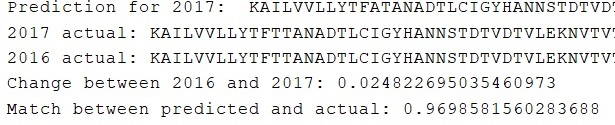
\includegraphics[width=\linewidth]{prediction1.jpg}
 \captionof{figure}{Example output}
\end{Figure}

Noting that our model wasn't accurate from a year-to-year basis, we were interested in investigating if there was any range of time that it became more accurate to use our model, as opposed to just assuming no change. One hypothesis was that the model might be more accurate at predicting change over longer periods of time than shorter periods of time. For example, predicting a year in the future was not found to be more accurate than assuming no change, but predicting 10 years in the future could be. We made to help visualize how much change had actually occurred since 1918, but ultimately this line of questioning was abandoned because it was decided that pursuing the question "when is our model incidentally right?" further would be be pointless. Regardless, here are complementary graphs made from when we thought the question might be relevant, included because they reveal interesting behavior of the influenza virus. 

\begin{Figure}
 \centering
 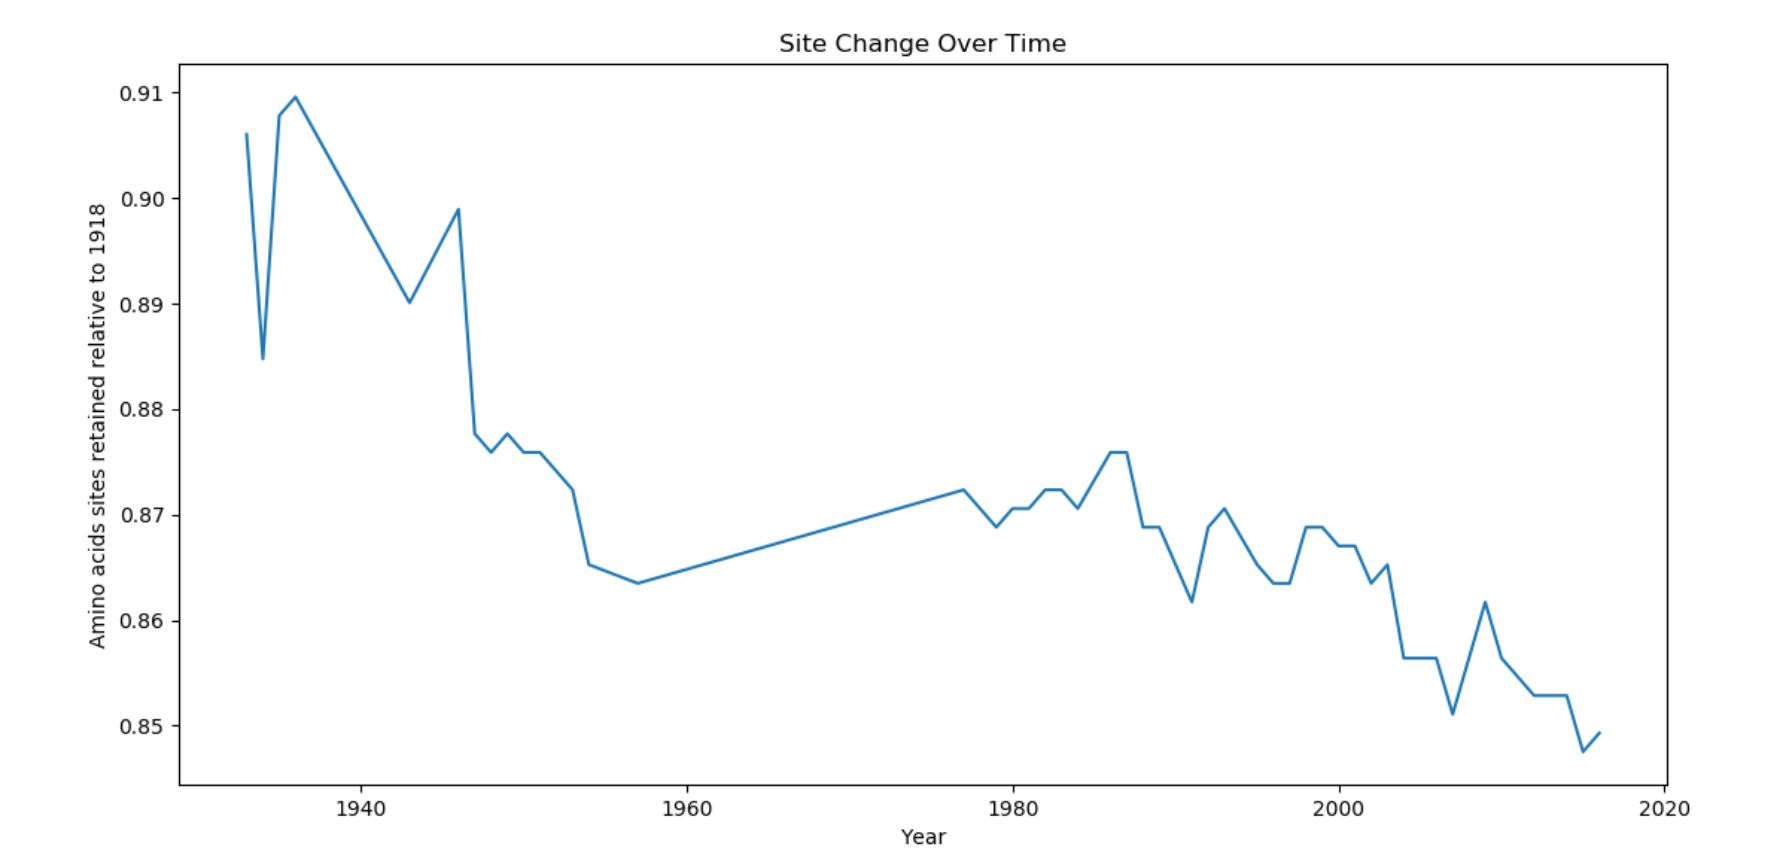
\includegraphics[width=\linewidth]{changeRelative1918.jpg}
 \captionof{figure}{Amino-acids retained, relative to 1918}
\end{Figure}

\begin{Figure}
 \centering
 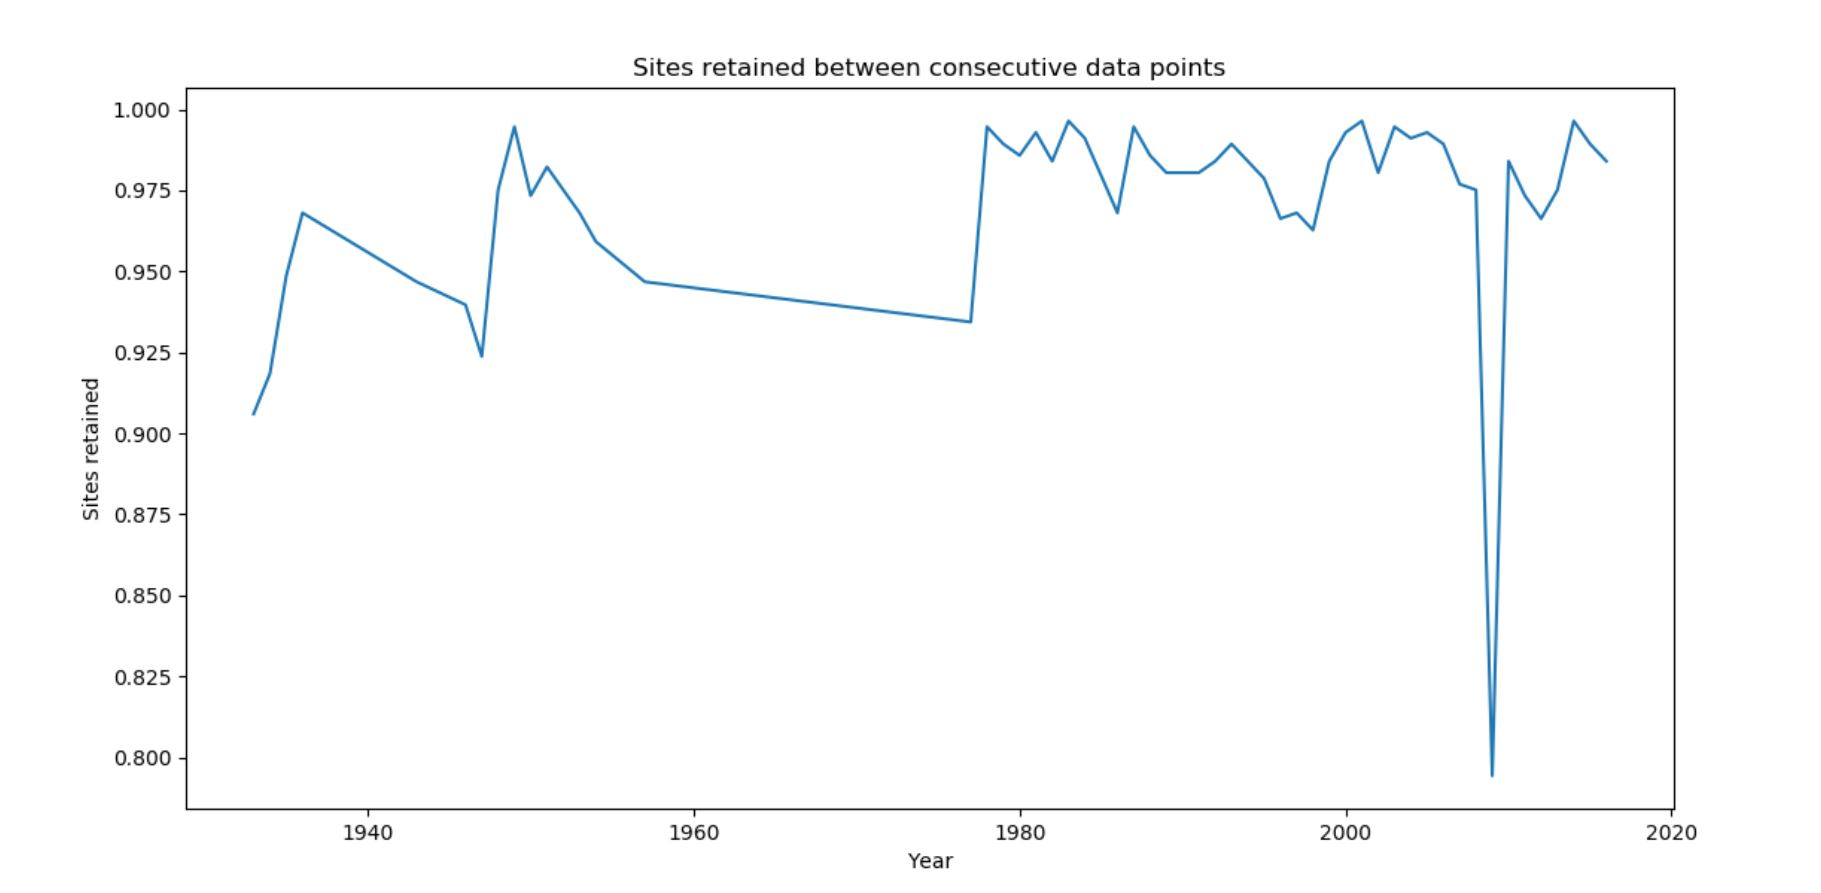
\includegraphics[width=\linewidth]{sitesretained.JPG}
 \captionof{figure}{Amino-acids retained between consecutive data points}
\end{Figure}

An exciting observation is the dip in amino-acids retained between 2008 and 2009. We believe that our analysis was able to detect the 2009 Swine flu outbrek, which lends credibility to our testing methods \citep{coburn2009modeling}.

\section{Results}
\subsection{Markov Chain}
Due to the stochastic element of our model, as well as the use of five different input data sets, the 2017 predictions for the DNA sequence of H1 Hemagglutinin slightly vary every time we run the model. Here is an example prediction for the 2017 DNA sequence of H1 Hemagglutinin:

\begin{Figure}
 \centering
 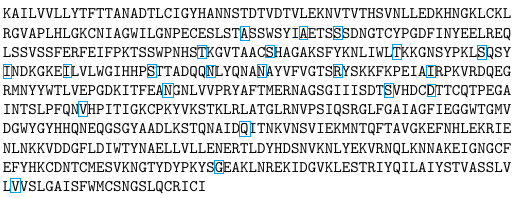
\includegraphics[width=\linewidth]{examplePrediction.PNG}
 \captionof{figure}{Example 2017 Prediction}
\end{Figure}

In Figure 8, we have highlighted the sites which differ from the actual 2017 DNA sequence of H1 Hemagglutinin. The actual 2017 DNA sequence of H1 Hemagglutinin is shown here in Figure 9:

\begin{Figure}
 \centering
 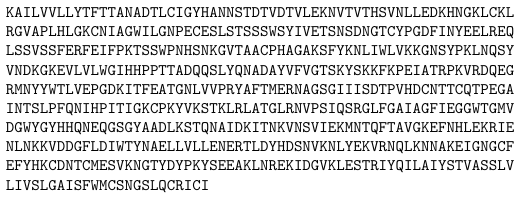
\includegraphics[width=\linewidth]{2017_actual.PNG}
 \captionof{figure}{2017 DNA Sequence}
\end{Figure}

This particular run of the model had about a 95.4\% matching rate to the actual sequence in 2017. More specifically, our model correctly predicted 544 out of 565 of the amino-acids in the 2017 sequence of H1 Hemagglutinin.

While our approach has not been previously performed, similar works which additionally incorporate insertions and deletions in their predictive model are able to succesfully predict the ``clade\footnote{A clade is phylogenetic grouping -- in this case, a clade refers to the specific strain of Influenza which will be prevalent (e.g., H1N1 or H3N2, etc.).}" of the following flu season \citep{luksza2014predictive}. The exact accuracy of these sequence predictions is reported to be between 96 and 99\%, however, the important implication is that the predictions are powerful enough to inform vaccine design. Other works are capable of perfectly predicting future sequences within one year, however, they are only accurate roughly 93\% of the time \citep{koelle2014influenza}. Given our relative lack of computational and experimental resources, we believe that the accuracy of our model is reasonable, considering that it's only marginally less powerful than leading models. However, we stress that our results are likely not powerful enough to inform vaccine design, as we may have made too many biological assumptions.

\subsection{Evolutionary Variability}

An important component of applying predictive models to vaccine design is investigating not just ``how" a virus is evolving, but also ``where". As part of our analysis, we also measured the ``evolutionary variability" of each site. Shown in figures 10 through 14 is the variability of each site relative to the overall structure of Hemagglutinin. This variability as shown as a color gradient from blue to red, with blue sites having the least variability. The sites in the highest variation class are highlighted as red spheres. The sites with high variation are generally located at the ``head", which is in-line with where it is expected to be according to past works from literature \citep{wiley1987structure}.
\begin{Figure}
 \centering
 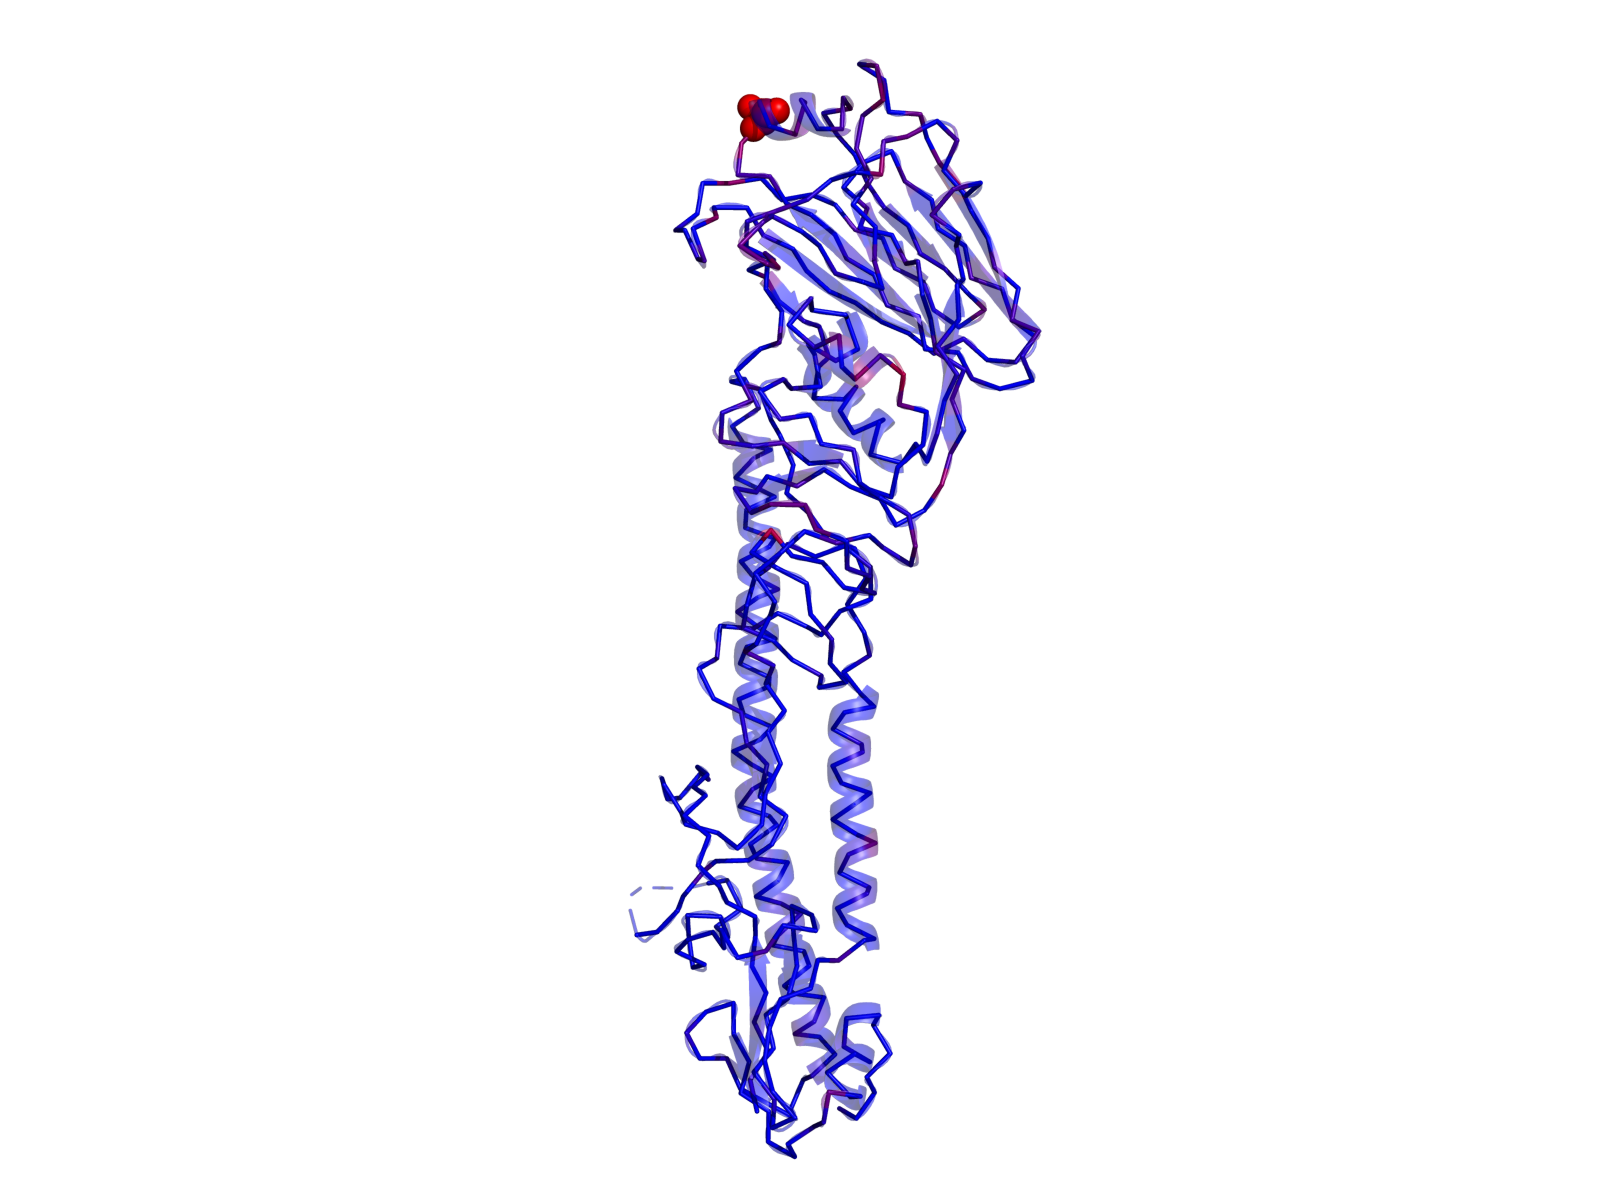
\includegraphics[width=\linewidth]{subsample_0_viewA.png}
 \captionof{figure}{Variation in the first data set.}
\end{Figure}
\begin{Figure}
 \centering
 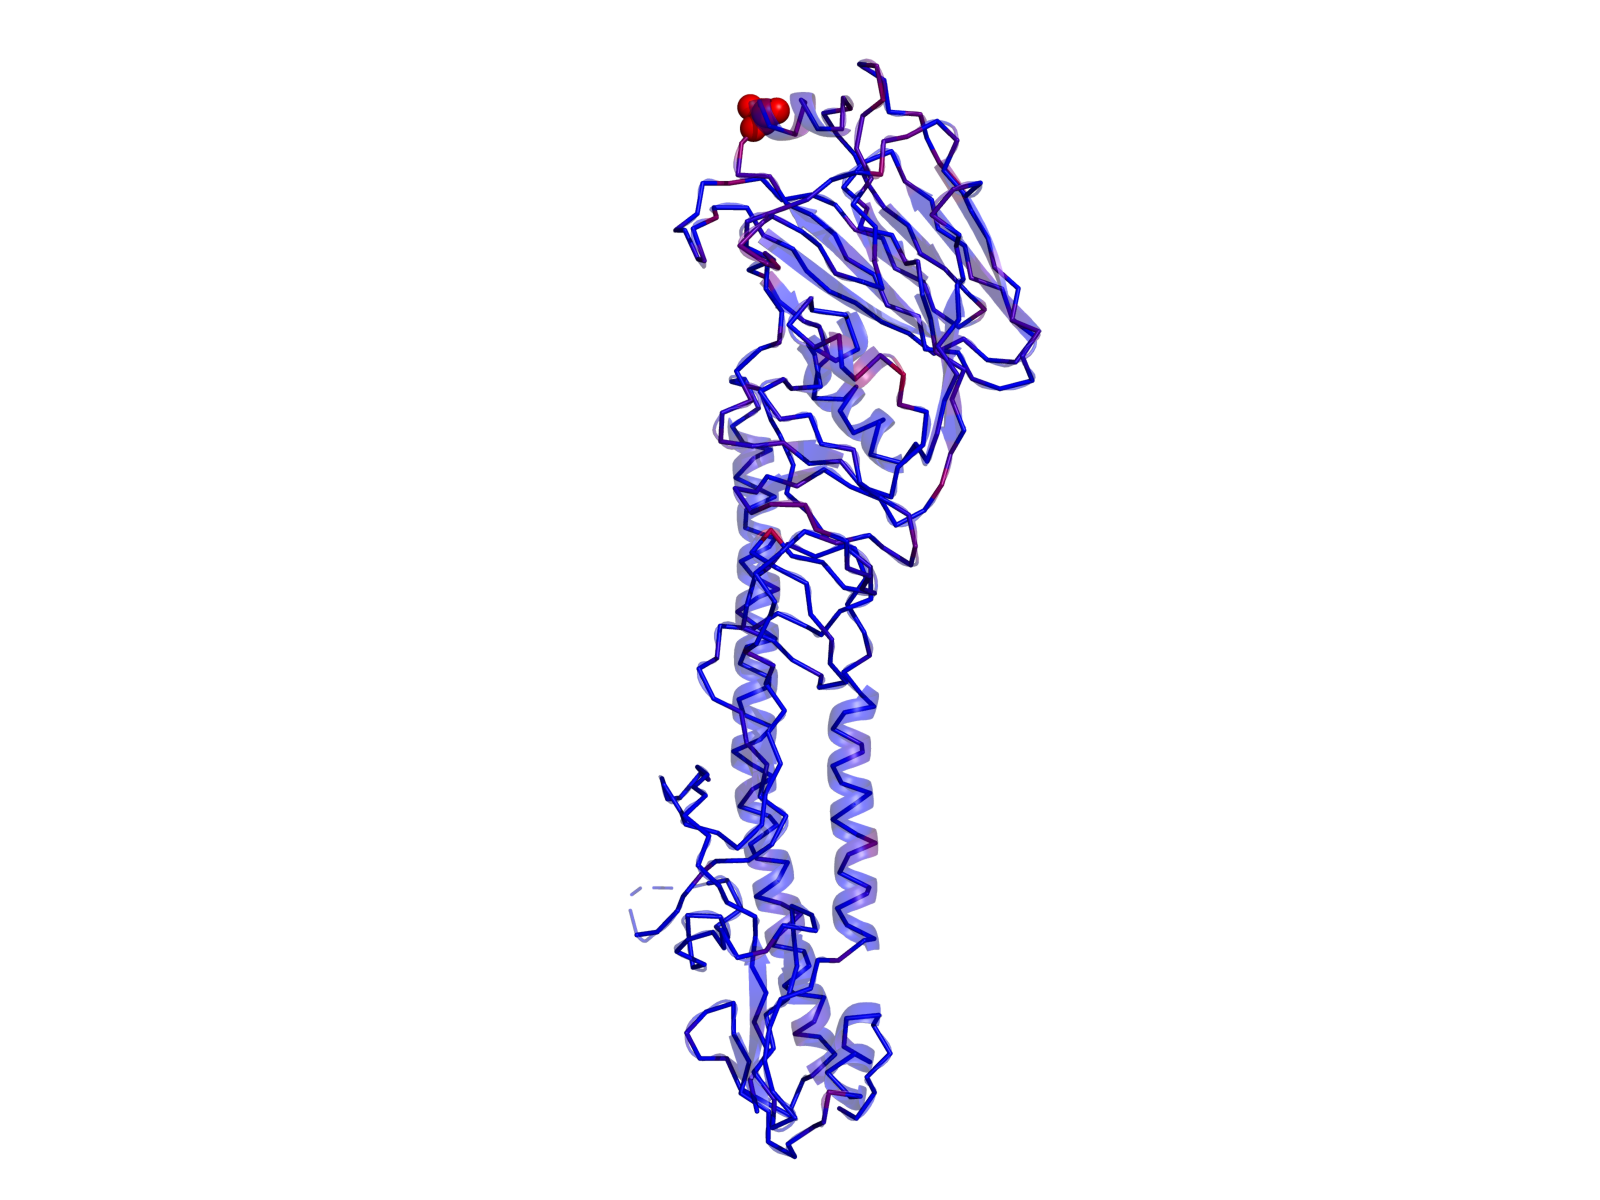
\includegraphics[width=\linewidth]{subsample_1_viewA.png}
 \captionof{figure}{Variation in the second data set.}
\end{Figure}
\begin{Figure}
 \centering
 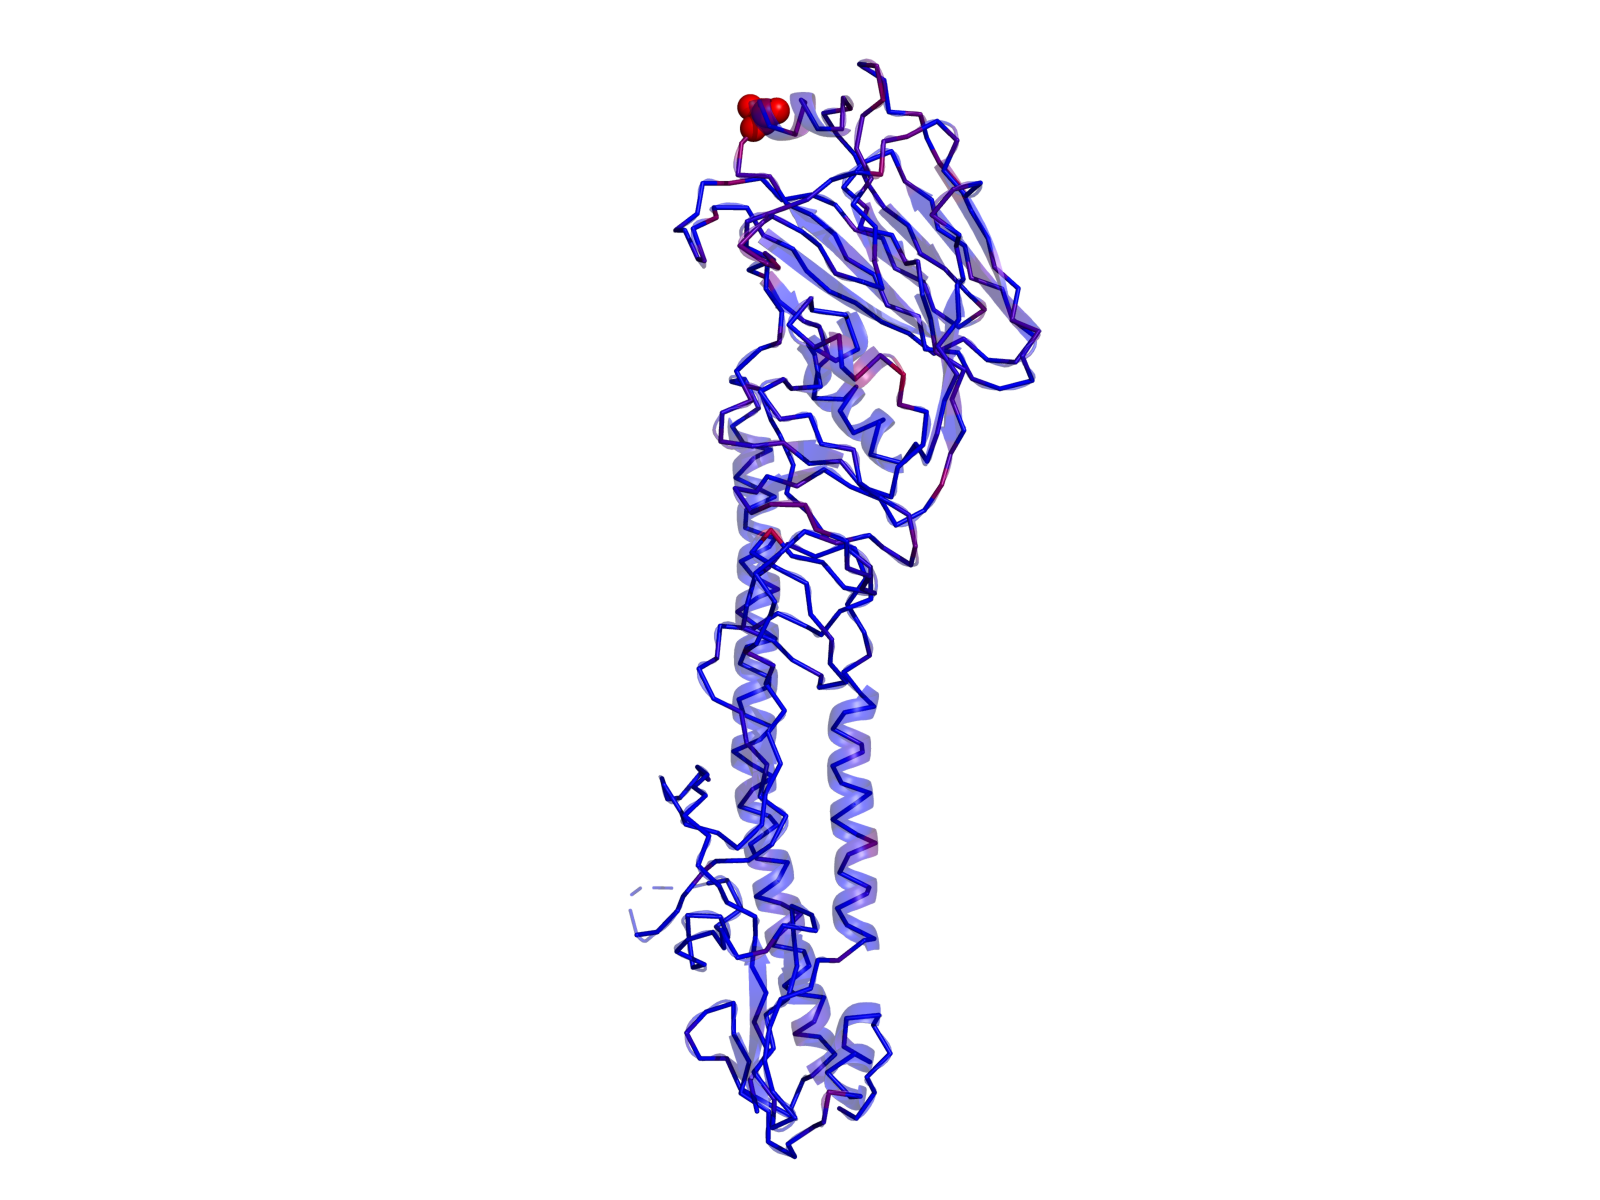
\includegraphics[width=\linewidth]{subsample_2_viewA.png}
 \captionof{figure}{Variation in the third data set.}
\end{Figure}
\begin{Figure}
 \centering
 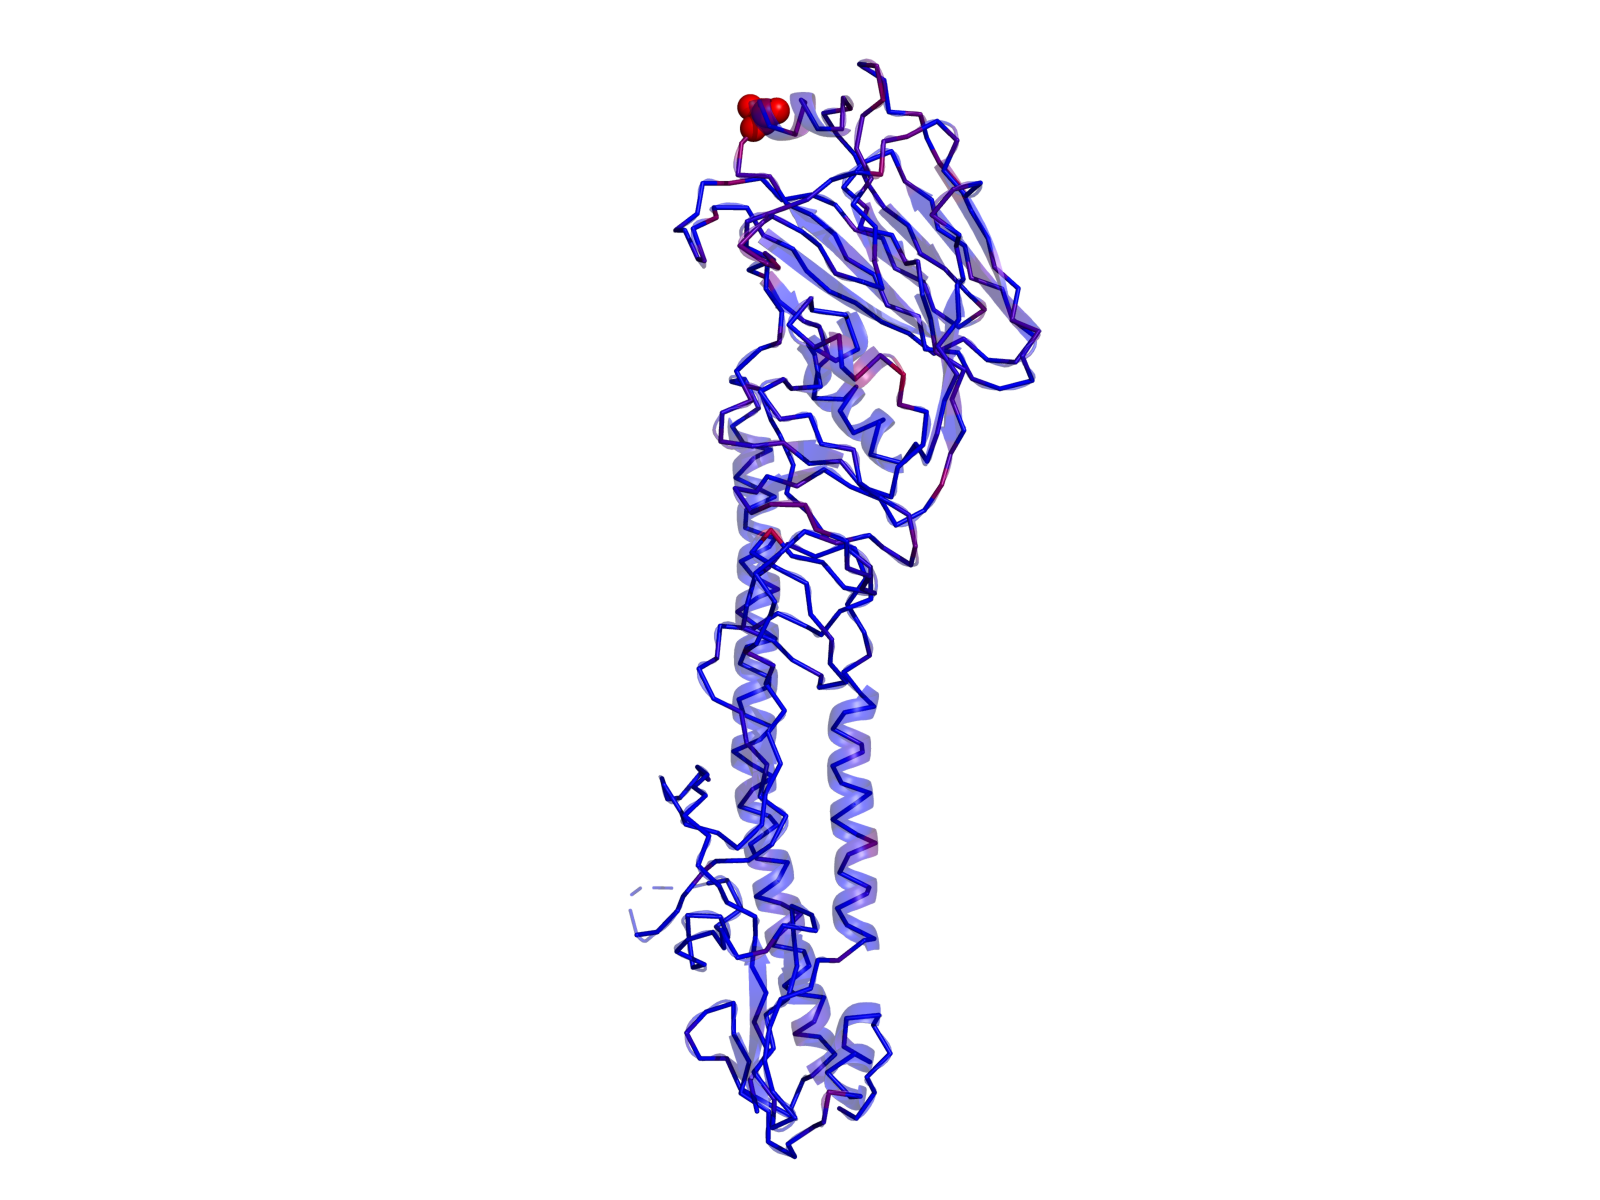
\includegraphics[width=\linewidth]{subsample_3_viewA.png}
 \captionof{figure}{Variation in the fourth data set.}
\end{Figure}
\begin{Figure}
 \centering
 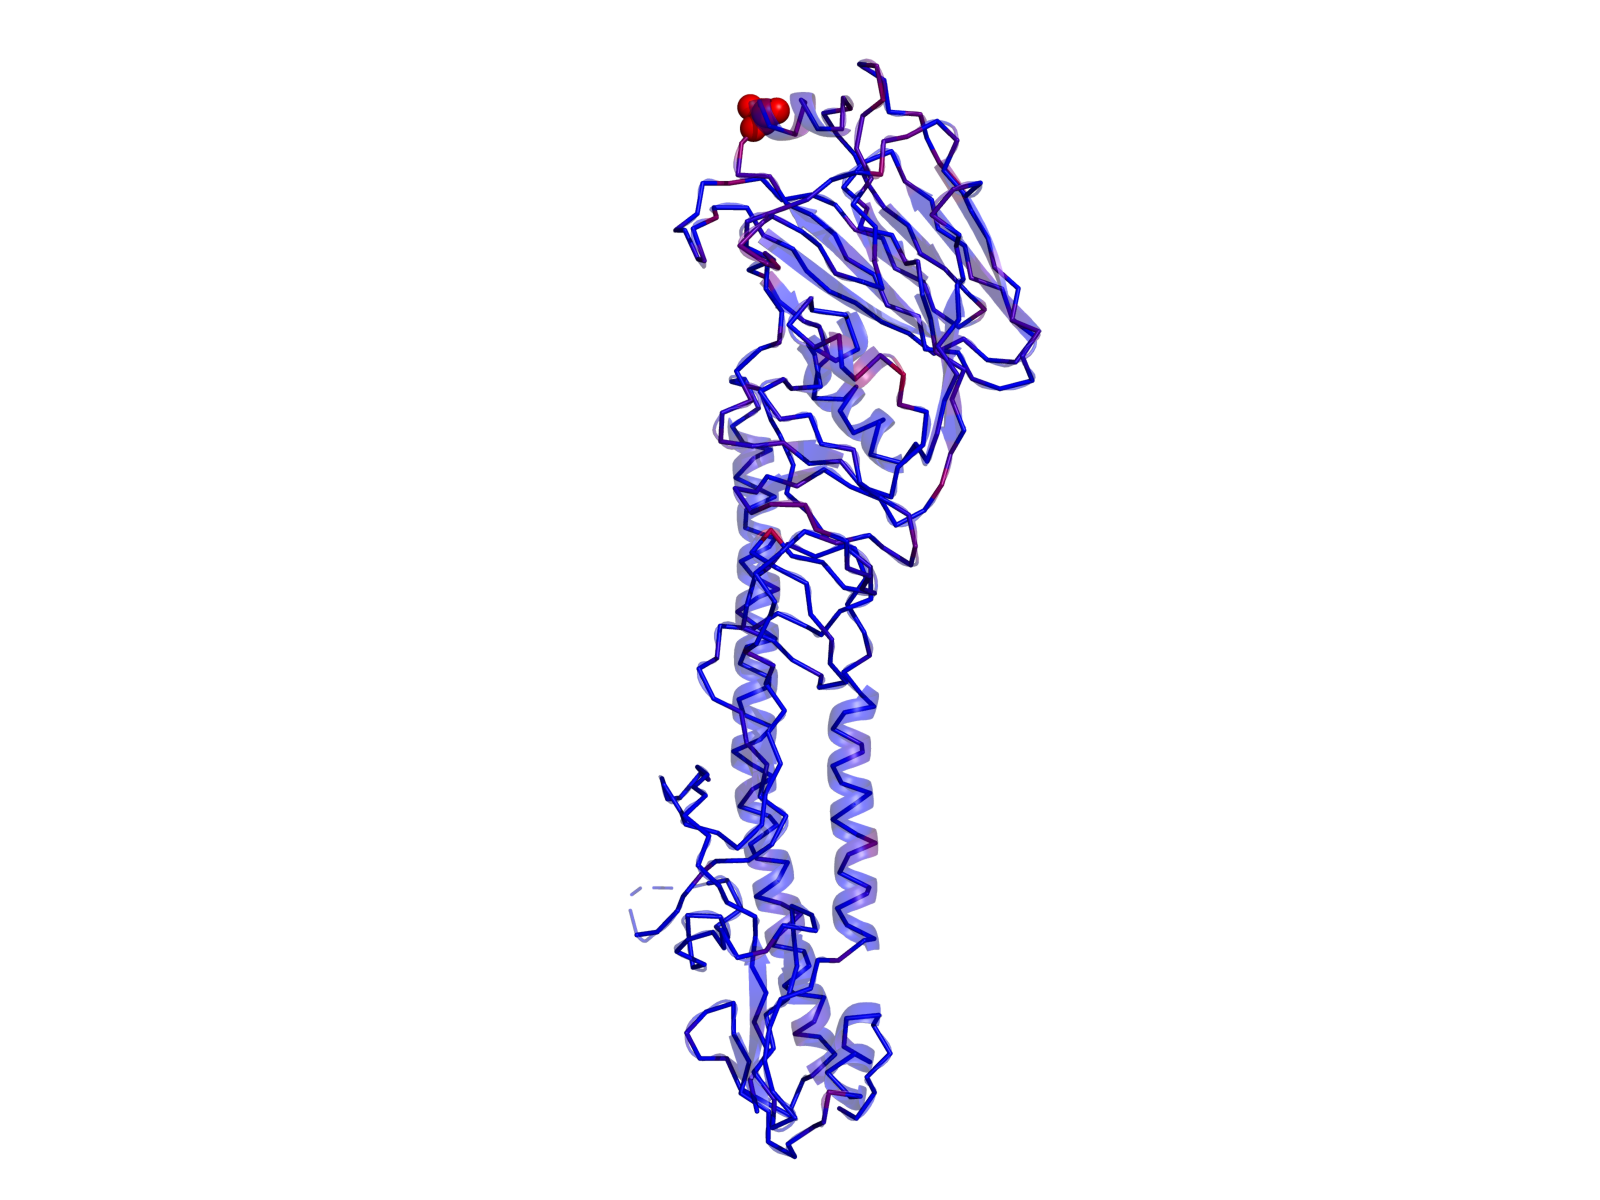
\includegraphics[width=\linewidth]{subsample_4_viewA.png}
 \captionof{figure}{Variation in the fifth data set.}
\end{Figure}

Notably, all five data sets appear to have similar variation between corresponding sites. More specifically, the site with the highest variation is consistent between all five data sets, being site 201.

In Figure 15, we have shown the location of known epitome locations\footnote{Epitope locations are where the immune system attacks viruses. These can experimentally identified in the lab, and H1 Hemagglutinin is particularly well studied.} on H1 Hemagglutinin as found in literature \citep{caton1982antigenic}. These sites were found to be under immune response, which means that they are expected to evolve ``faster" than expected\footnote{Sites that are under immune response will evolve faster in order to escape immune response.}. As a result, we would expect these sites to also have a high ``evolutionary variability", as accelerated evolution is typically due to increased selection pressure, which will also loosen functional and structural constraints \citep{wiley1987structure}.

\begin{Figure}
 \centering
 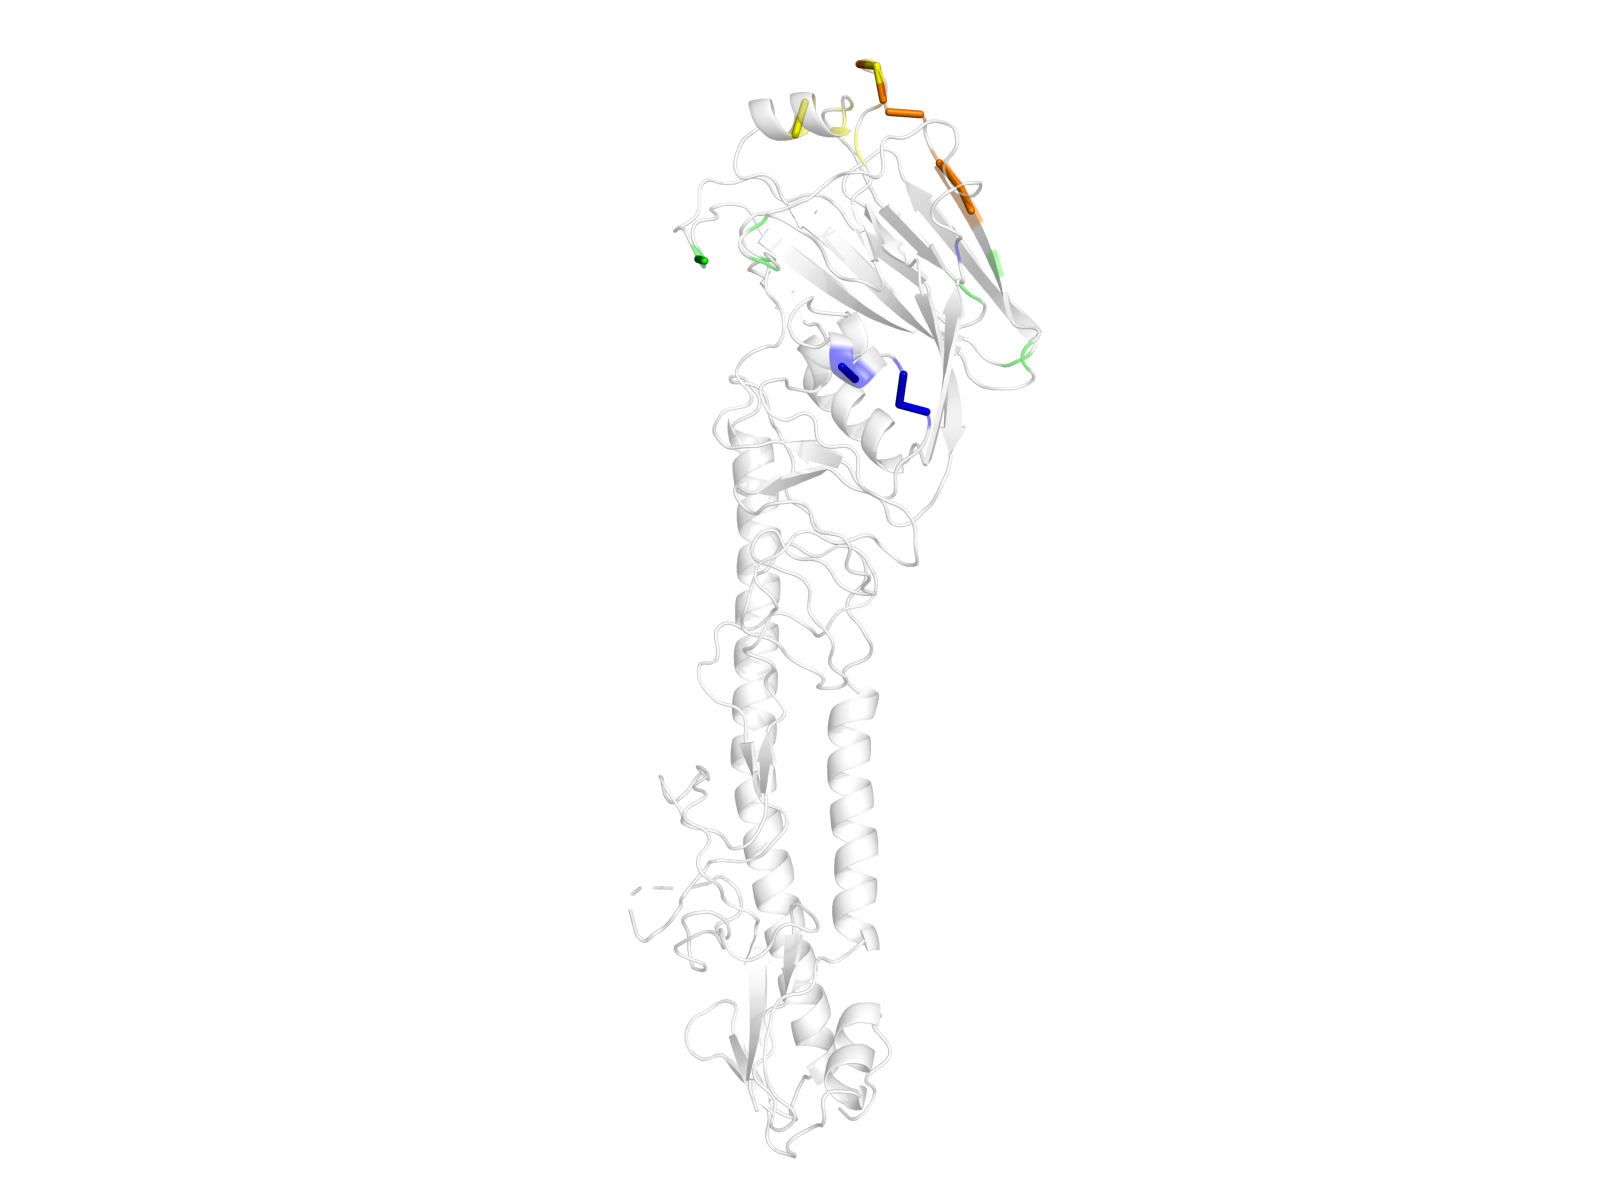
\includegraphics[width=\linewidth]{expEpi_viewA.png}
 \captionof{figure}{Variation from literature.}
\end{Figure}

More specifically, the known epitope regions are split into four distinct categories of sites, being:
\begin{verbatim}
Sa = [170, 172, 174, 175,
      177, 178, 179]
Sb = [168, 171, 204, 205,
      208, 210]
Ca = [181, 185, 219, 252,
      152, 155, 157, 236, 237]
Cb = [86, 87, 89, 90, 91,
      134]
\end{verbatim}

Notably, although there is no direct overlap between site 201 and the known epitope locations from literature, in both the experimental findings from literature as well as our model, it appears that most sites with high ``evolutionary variability" tend to be found in the top half of H1 Hemagglutinin. This suggests there is some moderate agreement between our computational methods and experimental findings from literature.

\section{Improvements}
As mentioned in the "Assumptions" section, we assumed that site changes were independent of each other. This seems unlikely in reality, and to improve our model, we could try to find correlations between different sites. For example, we could investigate how changes in site 6 could increase the likelihood that site 350 also changes, etc. A more "holistic" approach that factors in dependencies between sites would likely capture more of the evolutionary behavior, but would likely require more computational resources and a more complete data set. 

Similarly, as mentioned in \textit{Results}, other works which have successfully predicted influenza evolution to the extent of application to vaccine design have included other biological phenomena in their model \citep{luksza2014predictive}. These models included the ability to account for insertions and deletions, which was one of the assumptions that we ignored. It follows that a possible improvement to the model would be to incorporate insertions and deletions.

We first converted base pair sequences to amino-acids to construct the Markov probability matrix, with the assumption that amino-acids are more structurally relevant to proteins. The probability matrix was strictly based on site changes we saw from 1918 - 2016, but to supplement, we could look at the theoretical chance of individual DNA nucleotides changing, as opposed to amino-acids, so that we would insight towards what amino-acids could possibly be produced. For example, if given an DNA sequence that corresponds to Serine\footnote{DNA is read as length-3 sequences called ``codons". Each permutation of a codon results in an amino-acid, however, this translation is a surjective function, so different codons can code for the same amino-acid.} (TCC, for example), it is unlikely that it could switch to Valine (GTT, GTC, GTA, GTG) because it would require more than one base pair change in a single iteration \citep{brendel1986linguistics}. In a sense, this is similar to the "Word Ladder" game in class, and could be represented by a graph in which each edge is of length one, and there are 64 vertices representing the 64 codons\footnote{Permutations of length-3 sequences of DNA, which is in base-4, result in 64 unique codons.}. The distance between the codons ``TCC" and ``GTT", for example, would be at a minimum 3. Likely possible changes would be of a shorter distance. 

That being said, it seems unlikely that a theoretical approach to the problem could be an improvement over looking at the past 100-or-so years worth of data and making predictions based on empirical evidence. At most, it could probably supplement by giving a theoretical basis for what possible "spaces" the protein could evolve into. Evolutionary change is very incremental, so any changes that are retained would likely fall into the possible "spaces" predicted unless there is the unlikely scenario in which large changes at being made relatively quickly.  

\section{Conclusions}
Overall, our process does not not seem adequately suited for application to vaccine design, because it is ultimately a better prediction to assume that no change occurs from one year to the next.

There are a variety of possible explanations. Recall that there several assumptions made in designing the model, two of which were particularly relevant to our use of Markov chains: 1) that only the previous state influences the last state (this is the Markov property, also known as memorylessness), and 2), transition probabilities are not dependent on when the transitions occur (e.g., genetic continuity).

Based on the figures in the ``Testing" section, some fairly extreme changes occurred in 2008-2009 (and these changes can be directly connected to the swine flu virus). This suggests that the process might not be time-homogeneous (i.e., it's possible that the transition matrices are not the same as time passes) because a lot of change occurred within a relatively short period of time.

Another we made was that different sites are independent. Under this view, we focused on the primary structure of the protein\footnote{The primary structure of a protein is given by the sequence of amino-acids.}. However, the process in which a protein folds and coils upon itself\footnote{The folding of a protein is known as its secondary and tertiary structure.} is dependent on interactions that occur between nearby amino-acids. For this reason, it is somewhat inaccurate to assume that site changes are independent of each other because the interactions of different sites play an important role in determining the stability of a protein's structure.

Lastly, there was a huge amount of variation regarding transition possibilities. Below is an example of one of our outputs for a sequence. The first line represents transitions counted at site 1, the second line represents transitions counted at site 2, etc.

\begin{Figure}
 \centering
 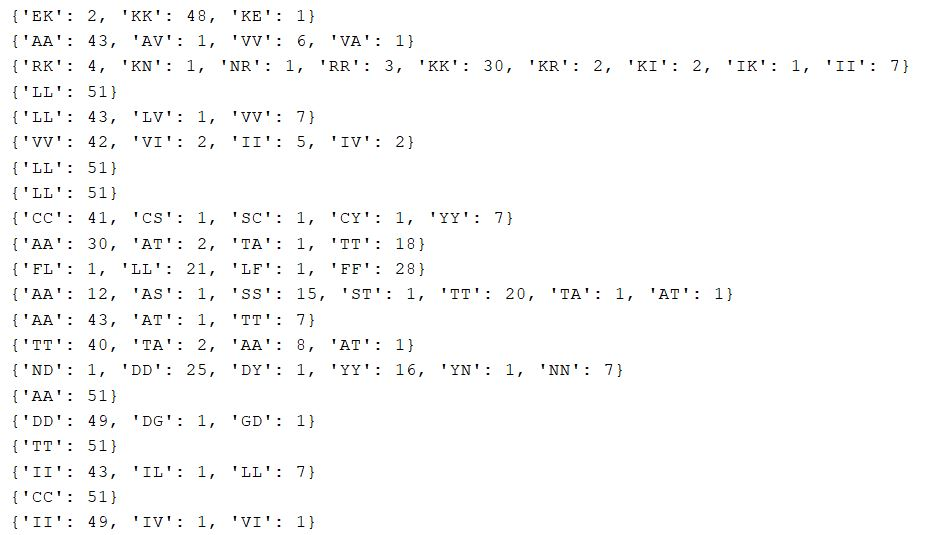
\includegraphics[width=\linewidth]{transitiondictionary.JPG}
 \captionof{figure}{Transitions per site}
\end{Figure}

As you can see, even when certain transitions are very common (for example, $K \rightarrow K$ for site 3), they might make up only slightly above 50\% of the possible transitions for a site -- meaning our prediction will have only slightly above a 50\% accuracy for that site. Likewise, if a given transition's probability represents the plurality but not the majority, then it's overall more likely for that transition to not occur.  

Stochastic modeling applied to evolutionary biology is not a new  concept. The Leslie process , used in modeling populations, was first described in 1945 \citep{leslie1945use}. The Moran process is a model proposed in 1958 that describes both variety-introducing processes like mutation, and variety reducing processes like natural selection and drift \citep{traulsen2005coevolutionary}. Our model improves upon past works in detecting the ``evolutionary space\footnote{The space available to Influenza evolution as given by its transitional probabilities and its variation class.}" that Influenza is capable of mutating towards, but due to this ``evolutionary space" being fairly large, specific predictions somewhat inaccurate. Further work is necessary to expand upon our findings before a Markov process can be adequately applied to predictive evolution and vaccine design.

\section{Acknowledgements}
E.B, G.J, and J.M contributed to the conceptualization and writing of the paper.
E.B and G.J were the primary contributors to the core mathematical modeling. 
J.M was the primary contributor to the structural and biological modeling. E.B was the primary contributor to comparing and evaluating the results.  G.J was the primary contributor to pipeline design. J.M was the primary contributor to literature research.

We made extensive use of the BioPython package \citep{cock2009biopython} and the PyMOL interface \citep{delano2002pymol}.

\end{multicols}
\newpage

\bibliographystyle{mbe}
\bibliography{references.bib}



\end{document}
